\documentclass{article}
\usepackage[utf8]{inputenc}

\title{Advanced Programming Labwork 9}
\author{Tom HERBRETEAU }
\date{November 2018}

\usepackage{natbib}
\usepackage{graphicx}
\usepackage{pgfplots}
\pgfplotsset{compat=newest}

\begin{document}

\maketitle
Every performance measures are done on ICT4 with eiffel.jpg, without counting the image saving.
\section{Introduction}
We have to compute the histogram of the input image, and use it to equalize this image.
\section{Implementation}
To compute the histogram, I choose to divide the input image into small blocks and compute a local histogram for each block. I use a structure to store arrays of histogram for all local histogram. The first kernel create an array of arrays for each local region, then the second kernel use REDUCE pattern to reduce to one histogram who contain the number of pixel of input image in total.
The next kernel will compute the CDF ton convert normal histo into equalized one, and the last kernel apply the equalized histogram to the output (MAP).
\section{Result}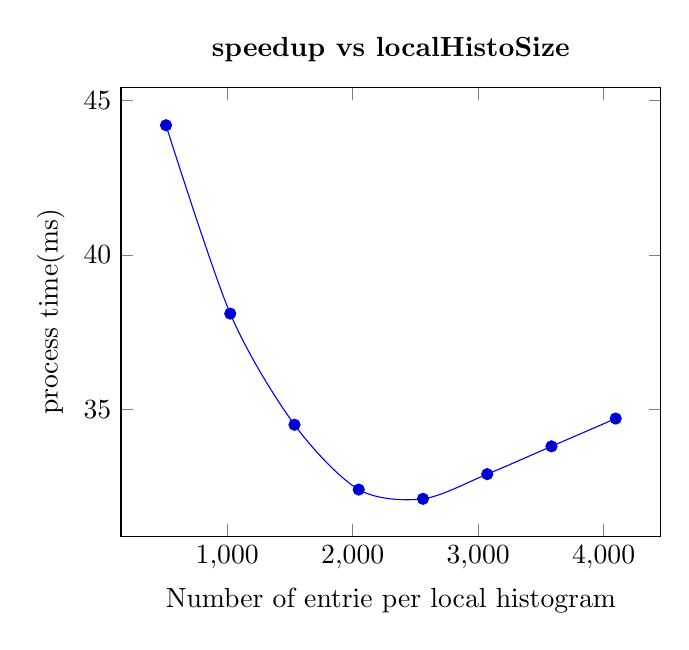
\begin{tikzpicture}
    \begin{axis}[title={\textbf{speedup vs localHistoSize}}, xlabel={Number of entrie per local histogram}, ylabel={process time(ms)}]
        \addplot+[smooth,mark=*] plot coordinates
            {(512, 44.2) (1024, 38.1) (1536, 34.5) (2048,32.4) (2560, 32.1) (3072,32.9) (3584,33.8) (4096, 34.7)};
    \end{axis}
\end{tikzpicture}
\newline
The program last around 32ms with the optimal parameter to process histogram and apply the equalization.
\newline
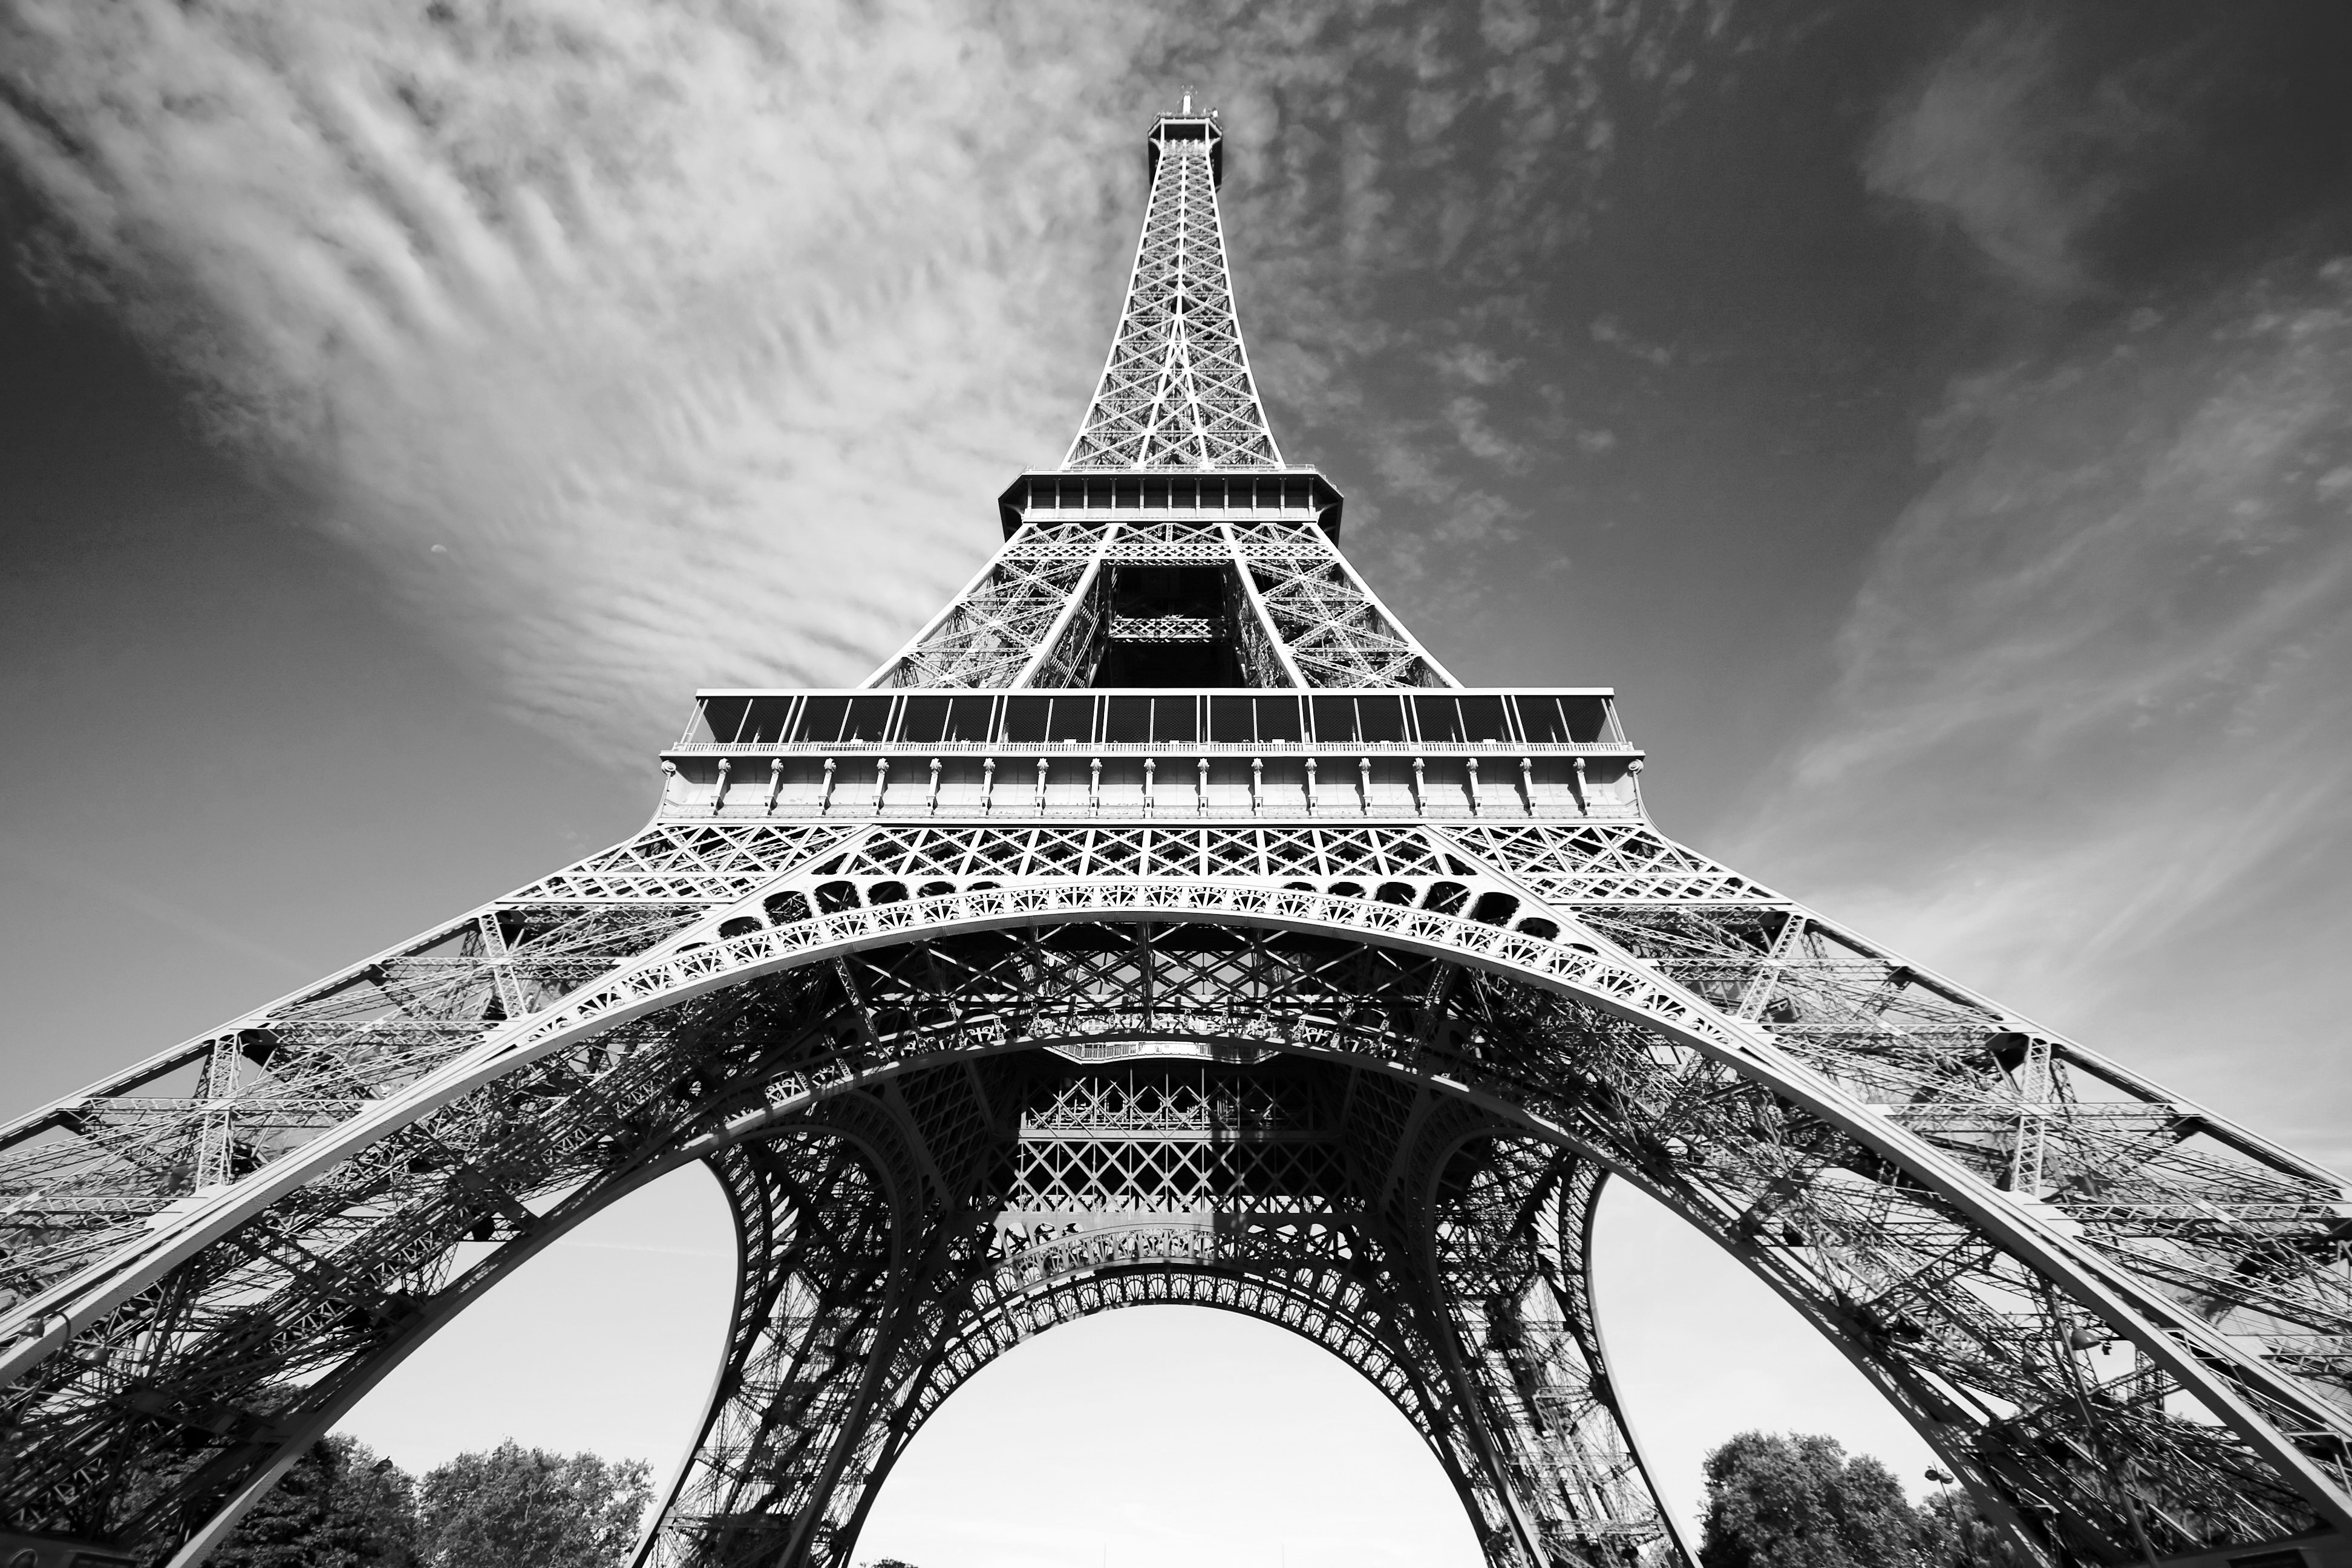
\includegraphics[width=\textwidth]{labwork9-gpu-out.jpg}
\bibliographystyle{plain}
\end{document}
